\setchapterpreamble[o]{
	\begingroup
	\vspace*{-2.60cm}\hspace*{-2.25cm}
	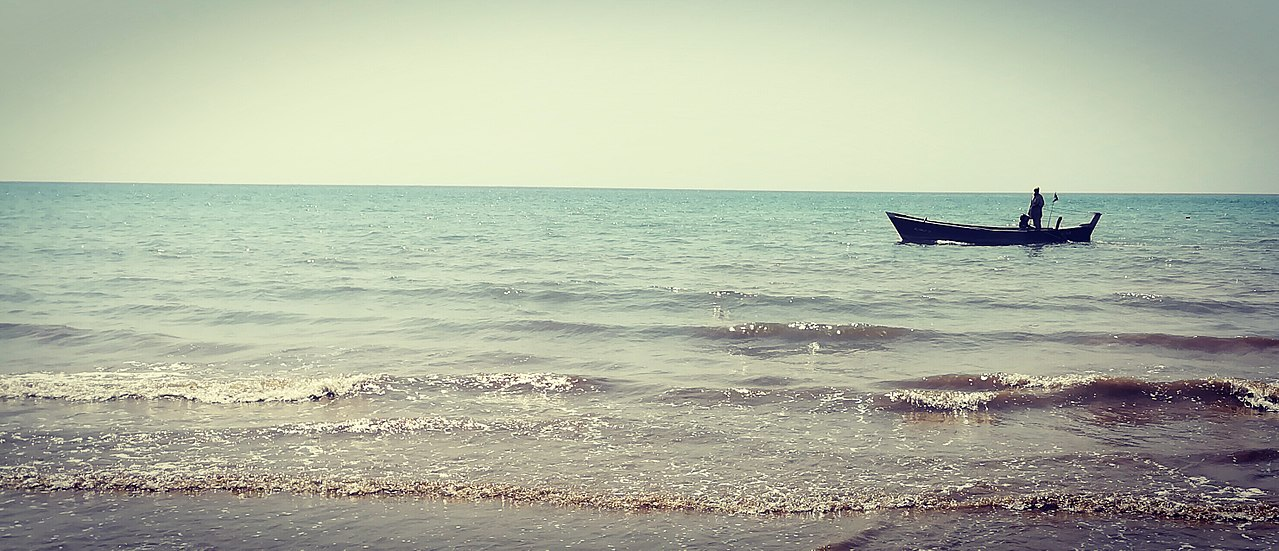
\includegraphics[width=\paperwidth,height=8cm,keepaspectratio=false]{images/seaside}
	\vspace{-1.0cm}
	\addtokomafont{captionlabel}{\bfseries}
	\captionsetup{
		type=figure,
		format=marginemph, 
		width=\textwidth+\marginparsep+\marginparwidth,
		%indention=2cm,
		parindent=0.7cm,
	}
	\caption[seaside]{By Bushra Feroz - Own work, CC BY-SA 4.0, 
		https://commons.wikimedia.org/w/index.php?curid=68724647}
	\endgroup
}
% beforeskip=-(figure_height-top_margin)
\RedeclareSectionCommand[beforeskip=-5.3cm]{chapter}
\setchapterpreamble[u]{\margintoc[*-6]}

\makeatletter
\renewcommand{\chapterlinesformat}[3]{%
  \@hangfrom{#2}{#3}%
}
\makeatother
\renewcommand*{\chapterformat}{%
  \mbox{\chapappifchapterprefix{\nobreakspace}\thechapter
	\autodot\IfUsePrefixLine{}{\enskip}}}

\chapter{Figures and Tables}
\RedeclareSectionCommand[beforeskip=0cm]{chapter}

\section{Normal figures and tables}

%\marginnote{\blindtext}

\blindtext

\begin{figure}[h]
	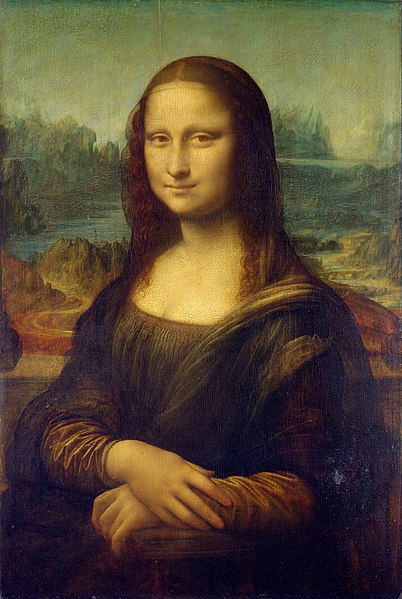
\includegraphics[width=0.4\textwidth]{monalisa}
	\caption{It's Mona Lisa again. \blindtext}
\end{figure}

\blindtext

\begin{table}
\begin{tabular}{ |c|c|c|c| } 
\hline
col1 & col2 & col3 \\
\hline
\multirow{3}{4em}{Multiple row} & cell2 & cell3 \\ 
& cell5 & cell6 \\ 
& cell8 & cell9 \\ 
\hline
\end{tabular}
\caption{A useless table. \blindtext}
\end{table}

\blindtext

\section{Margin figures and tables}

\blindtext

\begin{margintable}[*-6]
\begin{tabular}{ |c|c|c|c| } 
\hline
col1 & col2 & col3 \\
\hline
\multirow{3}{4em}{Multiple row} & cell2 & cell3 \\ 
& cell5 & cell6 \\ 
& cell8 & cell9 \\ 
\hline
\end{tabular}
\caption{A useless table.}
\end{margintable}

\section{Wide figures and tables}
